\documentclass[a4paper,12pt,twoside]{report}

\usepackage[french]{babel}  % Pour le français
\usepackage[utf8]{inputenc} % Pour taper les caractères accentués
\usepackage[T1]{fontenc} %Not needed on school computers

\usepackage{amsmath}  % Ces trois paquets donnent accès à 
\usepackage{amsfonts} % des symboles et formulations 
\usepackage{amstext}  % mathématiques
\usepackage{hyperref} % Permet de faire automatiquement des liens dans les
                      % documents
\usepackage{graphicx} % Permet d'insérer des images
\DeclareGraphicsExtensions{.png} % Mettre ici la liste des extensions des
                                 % fichiers images

% On peut choisir la police en utilisant un paquet 
%\usepackage{newcent}
\usepackage{lmodern}
%\usepackage{cmbright} % Computer Modern Bright

% Une des nombreuses manière de modifier les marges par défaut
\usepackage{geometry}
\geometry{vmargin=2cm,hmargin=2.5cm,nohead}

% If si units are needed : \usepackage{siunitx}

% On peut redéfinir certaines longueurs, par exemple l'espacement entre les
% paragraphes:
\setlength{\parskip}{0.25cm}

% Quelques définitions 
\def \rr {{\mathbb R}} % L'ensemble R
\def \cc {{\mathbb C}} % L'ensemble C
\def \nn {{\mathbb N}} % L'ensemble N
\def \zz {{\mathbb Z}} % L'ensemble Z

% Les informations de la page de titre (page de titre séparée pour un 'report').
\title{
\vspace*{1in}
\textbf{Electrocardiogramme}}

\author{Rémi HERNANDEZ\\
        Romuald MAKOSSO NOMBO\\
        Amandine CAUT\\
        Célia BOULTABI\\
		\vspace*{0.5in} \\		
		Tuteur : Y.Courdiere \\	
		\vspace*{0.5in} \\		
		Université de Bordeaux\\		
       } 
%--------------------Make usable space all of page
\setlength{\oddsidemargin}{0in} \setlength{\evensidemargin}{0in}
\setlength{\topmargin}{0in}     \setlength{\headsep}{-.25in}
\setlength{\textwidth}{6.5in}   \setlength{\textheight}{8.5in}
%--------------------Indention
\setlength{\parindent}{1cm}


% \thanks: permet de mettre une note de bas de page pour l'auteur
% \href: insère un lien, ici vers l'application 'mailto'
% \tt: police monospace
\date{\today} % \today pour la date courante 

\cleardoublepage

\begin{document}

\maketitle % Page de titre automatique à partir des infos ci-dessus

% La commande cleardoublepage est utilisée pour s'assurer que la page suivante
% est une page de droite lorque l'on imprime recto-verso.



\pagebreak
\hspace{0pt}

\vfill
\hspace{0pt}
\pagebreak




\cleardoublepage
\tableofcontents % Table des matière automatique à partir des chapitres,
                 % sections, etc du document



\chapter{Étude théorique} 

L'électrophysiologie permet de modéliser la propagation de différentes ondes dans le cœur. \\
Pour cela nous allons utiliser cette équation:\\

$$\partial_t u(x,t) - \partial_x(a(x) \partial u(x,t)) = f(t,x)$$

Afin de résoudre cette équation il faut certaines conditions initiales et aux bords. Nos recherches dans différents livres et articles nous permettent alors de déduire les conditions suivantes: \\
\\
$$ 
\left\{ 
	\begin{array}{ll}
		\partial_t u(x,t) - \partial_x(a(x) \partial u(x,t)) = f(t,x) \\
		a(x) \partial_x u(x,t) = 0 \ sur \  \partial \Omega\\
		u(0,x) = u_0(x) \ t \in [0,T]
		
	\end{array}
\right. 
$$


Il est nécessaire que $a(x) > 0$, afin que le phénomène ne soit pas réversible! En effet, on ne peut inverser la diffusion de la chaleur. \\ 
On remarque par ailleurs que l'on a l'équation chaleur pour le cas $a(x) = 1$. On résoudra cette équation dans le chapitre 2.








Situation où l'on peut calculer des solutions analytiques: \\
dans le cas ($a(x) = 1$) on a l'équation de la chaleur. De plus avec nos conditions aux bords, ie les dérivées sont nulles, on a deux cas, $ f(x) \neq 0$ ou $f(x) = 0$. Ici, on prend le cas où $f(x) = 0$: \\
 


la solution est la fonction u définie par : \\
$$ u(x,t) =  cos(k \pi x) exp(-k^2 \pi^2 t) $$ 



Résolution du cas: \\
Nous allons résoudre le système par la méthode de séparation des variables.\\
On pose u(x,t) = f(x)g(t)\\
de ce fait: 
$$\partial_t u(x,t) = f(x)g'(t) $$ et $$\partial_{xx}^2 u(x,t) = f(x)''g(t)$$ \\
On obtient : \\
$$ \frac{g'(t)}{g(t)} = \frac{f''(x)}{f(x)} = c $$ \\
Et donc: 
$ g(t) = \lambda exp(ct) $ avec c < 0 sinon la solution explose ce qui est impossible.\\
$$\frac{f''(x)}{f(x)} = c \Leftrightarrow f''(x) - cf(x) = 0$$ \\
$$ \Leftrightarrow f(x) = P cos(x \sqrt{|c|}) + Qsin(x \sqrt{|c|})$$ \\
par compilation on a alors, \\
$$ u(x,t) = \lambda exp(ct) (P cos(x \sqrt{|c|}) + Qsin(x \sqrt{|c|})) $$ \\
or $\partial_x u(x,t) = 0 \ sur \  \partial \Omega$, donc on dérive l'expression et on remplace: \\
$$ -P \sqrt{|c|} sin(x \sqrt{|c|}) + Q \sqrt{|c|} sin(x \sqrt{|c|}) = 0$$ \\

On obtient le système de résolution suivant: 

$$
\left\{
	\begin{array}{ll}
		x = 0 \Leftrightarrow Q \sqrt{|c|} sin(x \sqrt{|c|}) = 0\\
		x= 1 \Leftrightarrow -P \sqrt{|c|} sin(x \sqrt{|c|}) = 0

	\end{array}
\right. 
$$


$$
\Leftrightarrow
\left\{
	\begin{array}{ll}
		x = 0 \Leftrightarrow Q = 0 $$ \; car \;c < 0 $$\\
		x= 1 \Leftrightarrow sin(x \sqrt{|c|}) = 0 $$ \; car \; P \neq 0 $$

	\end{array}
\right. 
$$\\
 On obtient ainsi: $c= (k \pi)^2 \; \forall k \in \mathbb{Z} $ \\
La solution s'écrit donc $ u(x,t) = \lambda exp((k \pi)^2t $ , avec la condition initiale $u(0,x) = u_0 (x)$ on a alors $u_0 (x) = cos(xk \pi)$ avec $\lambda = 1$.

\chapter{programmation dans un cas simplifié} 
\section{Schémas numériques pour la résolution}

Pour la résolution de cette équation, on utilise un maillage uniforme avec un pas de $\Delta t$ en temps et $\Delta x$ en espace. \\
La dérivée seconde en espace est approchée par : 
\begin{equation}
\frac{\partial ^2u}{\partial ^2x} = \frac{u(x_{i+1},t_j) - 2u(x_i,t_j) + u(x_{i-1},t_j)}{\Delta x^2}
\end{equation}

\subsection{Euler explicite}

On approche $\frac{\partial u}{\partial t}(x_i,t_j)$ par :
\begin{equation}
\frac{u(x_i,t_j+1) - u(x_i,t_j)}{\Delta t}
\end{equation}
On obtient le schéma suivant :\\
\begin{equation}
\frac{u(x_i,t_j+1) - u(x_i,t_j)}{\Delta t} - \frac{u(x_{i+1},t_j) - 2u(x_i,t_j) + u(x_{i-1},t_j)}{\Delta x^2} = f(x_i,t_j)
\end{equation}
Pour la suite on écrira $u^j_i$ à la place de $u(x_i,t_j)$. \\ 
Aussi on utilisera la notation :
$U^j = \left( \begin{array}{c}
u^j_0\\
u^j_1 \\
\vdots \\
u^j_N
\end{array} \right)$

Le schéma s'écrit sous forme matricielle :
\begin{equation}
\frac{U^{j+1}-U^j}{\Delta t} + A_{\Delta x}U^j = F^j
\end{equation}
Avec :
\begin{equation}
A_{\Delta x} = \frac{1}{\Delta x^2}
\begin{pmatrix}
   2 & -1 & 0 & \ldots & \ldots & 0\\
   -1 & 2 & -1 & 0 \ddots & & \vdots \\
   0 & \ddots & \ddots & \ddots & \ddots & \vdots\\
   \vdots & \ddots & \ddots & \ddots &\ddots & 0\\
   \vdots & & \ddots & -1 & 2 & -1\\
   0 & \cdots & \cdots & 0 & -1 & 2
\end{pmatrix}
\end{equation}
Et on a $F^j = \left( \begin{array}{c}
f(x_1,t_j)\\
f(x_2,t_j) \\
\vdots \\
f(x_N,t_j)
\end{array} \right)$


\smallbreak
Par les formules de Taylor, on discrétise la dérivée seconde en espace:\\
$$f(x + \Delta x, t) = f(x,t) + \Delta x \partial_x f(x,t) + \frac{(\Delta x)^2}{2} \partial_{xx} ^2 f(x,t) + \theta (\Delta x^3) $$ \\

$$f(x - \Delta x, t) = f(x,t) - \Delta x \partial_x f(x,t) + \frac{(\Delta x)^2}{2} \partial_{xx} ^2 f(x,t) + \theta (\Delta x^3) $$ \\
On soustrait les deux équations: \\

$$f(x + \Delta x, t) -f(x - \Delta x, t) = 2 \Delta x \partial_x f(x,t) + \theta (\Delta x^3) $$ \\
$$\frac{f(x + \Delta x, t) -f(x - \Delta x, t)}{2 \Delta x} = \partial_x f(x,t) + \theta (\Delta x^2)$$ \\
$$\partial_x f_k ^n = \frac{f_{k+1} ^n - f_{k-1} ^n}{2 \Delta x}$$ \\


On effectue le même raisonnement que précédemment pour trouver la dérivée seconde:\\
$$ \partial_x(a(x) \partial_x u(x,t)) = \frac{1}{ \Delta x}(a_{k+\frac{1}{2}} \partial_x u_{k+\frac{1}{2}} ^n - a_{k-\frac{1}{2}} \partial_x u_{k-\frac{1}{2}} ^n) $$\\

On remplace dans l'équation de la dérivée seconde ce que l'on a trouvée pour la dérivée première:\\
$$\partial_x(a(x) \partial u(x,t))_k ^n= \frac{1}{ \Delta x} (a_{k+\frac{1}{2}} (\frac{u_{k+1} ^n - u_{k} ^n}{ \Delta x})- a_{k-\frac{1}{2}} (\frac{u_{k} ^n - u_{k-1} ^n}{ \Delta x}))$$ \\
On factorise par $\frac{1}{\Delta x}$ , ce qui donne: \\
$$\partial_x(a(x) \partial u(x,t))= \frac{1}{( \Delta x)^2} (a_{k+\frac{1}{2}} u_{k+1}^n - 
(a_{k+\frac{1}{2}} +a_{k-\frac{1}{2}}) u_k ^n +
a_{k-\frac{1}{2}}u_{k-1} ^n )$$\\

On discrétise la dérivée en temps par $\frac{u_{k} ^{n+1} - u_{k} ^n}{ \Delta t}$, de ce fait on a le système suivant: \\

Pour $n \in [0, J]$ et $k \in [1, N-1]$, avec $J = \frac{T}{\Delta t} $ et $N = \frac{1}{\Delta x}$, on a: \\

$$ 
\left\{ 
	\begin{array}{ll}
		\frac{u_{k} ^{n+1} - u_{k} ^n}{ \Delta t} - \frac{1}{( \Delta x)^2} (a_{k+\frac{1}{2}} u_{k+1}^n -(a_{k+\frac{1}{2}} +a_{k-\frac{1}{2}}) u_k ^n + a_{k-\frac{1}{2}}u_{k-1} ^n ) = f_k ^n \\
		a(x) \partial_x u_0 ^n = 0 \leftrightarrow \partial_x u_0 ^n = 0  \\
		\partial_x u_N ^n = 0\\
		a_N \partial_x u_N ^n = 0
		
		
	\end{array}
\right. 
$$

On isole le $u_k ^{n+1}$:\\
$$u_k ^{n+1} = \frac{\Delta t}{ \Delta x ^2} (a_{k+\frac{1}{2}} u_{k+1}^n -(a_{k+\frac{1}{2}} +a_{k-\frac{1}{2}}) u_k ^n + a_{k-\frac{1}{2}}u_{k-1} ^n ) + f_k ^n + u_k ^n$$
On regroupe les termes $u_k ^n$,  $ u_{k-1} ^{n}$ et $ u_{k+1} ^{n}$ :\\
$$u_k ^{n+1} = \frac{\Delta t}{ \Delta x ^2} a_{k-\frac{1}{2}} u_{k-1} ^n +(1- \frac{\Delta t}{\Delta x^2} (a_{k-\frac{1}{2}} + a_{k+\frac{1}{2}}))u_k ^ n +\frac{\Delta t}{\Delta x^2} a_{k+\frac{1}{2}} u_{k+1} ^n + f_k ^n$$
D'après les conditions au bord, on a:\\
$$
\left\{
	\begin{array}{ll}
		\partial_x(a(x) \partial u(x,t))_0 ^n = \frac{2}{\Delta x} a_{\frac{1}{2}} \partial_x u_{\frac{1}{2}} ^n = \frac{2}{\Delta x} a_{\frac{1}{2}} \frac{u_1 ^n - u_0 ^n}{\Delta x} \\
		\partial_x(a(x) \partial u(x,t))_N ^n = 0 -\frac{a_{N-\frac{1}{2}} \partial_x u_{N-\frac{1}{2}} ^n}{\frac{\Delta x}{2}} = -\frac{2}{\Delta x} a_{N-\frac{1}{2}} \frac{u_N ^n - u_{N-1}^n}{\Delta x}

	\end{array}
\right. 
$$
De ce fait l'équation discrétisée au bord donne: \\
$$\frac{u_{k} ^{n+1} - u_{k} ^{n}}{ \Delta x} - \frac{2}{( \Delta x)^2} a_{N-\frac{1}{2}}(\frac{u_N ^n - u_{N-1}^n}{\Delta x})  = f_k ^n$$
pour k= 0: $\frac{u_{0} ^{n+1} - u_{0} ^{n}}{ \Delta x} - \frac{2}{( \Delta x)^2} a_{\frac{1}{2}}(u_1 ^n - u_0^n)  = f_0 ^n$ \\

On isole $u_0 ^{n+1}$: $u_0 ^{n+1} = \frac{2 \Delta t}{ \Delta x ^2} a_{\frac{1}{2}} (u_1^n -u_0 ^n) + f_0 ^n + u_0 ^n$ \\

Puis, $u_0 ^{n+1} = u_0 ^{n} - \frac{2 \Delta t}{ \Delta x ^2} a_{\frac{1}{2}} u_0 ^n + \frac{2 \Delta t}{ \Delta x ^2} a_{\frac{1}{2}} u_1 ^n + f_0 ^n$ \\

\bigbreak


Finalement, l'équation s'écrit pour $k = 0,...N$ et $n = 1,...,J$:


$$
\left\{
	\begin{array}{ll}
		u_k ^{n+1} = u_k ^{n} + \frac{ \Delta t}{ \Delta x ^2} a_{k - \frac{1}{2}} u_{k-1} ^n - \frac{ \Delta t}{ \Delta x ^2} ( a_{k + \frac{1}{2}} +a_{k - \frac{1}{2}}) u_{k} ^n +\frac{ \Delta t}{ \Delta x ^2} a_{k+ \frac{1}{2}} u_{k+1} ^n + f_k ^n\\
		u_k ^{n+1} = u_k ^{n} +  \frac{2 \Delta t}{ \Delta x} a_{n - \frac{1}{2}} u_{N-1} ^n -  \frac{2 \Delta t}{ \Delta x} a_{n - \frac{1}{2}} u_{N} ^n + f_N ^n
	\end{array}
\right. 
$$\\
avec $u^n = (u_0 ^n, u_1 ^n, ...u_N ^n) $ et $ F^n = (f_0 ^n, f_1 ^n, ...f_N ^n)$ \\
On écrit cela sous forme matricielle:\\
$$U^{n+1} = U^n - \frac{\Delta t}{ \Delta x^2} AU^n + F^n \Delta t$$ \\

On obtient alors la matrice suivante: \\

\begin{equation}
A = 
\begin{pmatrix}
   2 a_{\frac{1}{2}} & -2 a_{\frac{1}{2}} & 0 & \ldots & \ldots & 0\\
   -a_{\frac{1}{2}} & - (a_{\frac{1}{2}} + a_{\frac{3}{2}} ) & -a_{\frac{3}{2}} & 0 \ddots & & \vdots \\
   0 & -a_{\frac{3}{2}} & - (a_{\frac{5}{2}} + a_{\frac{3}{2}} ) & -a_{\frac{5}{2}} & \ddots & \vdots\\
   \vdots & \ddots & \ddots & \ddots &\ddots & 0\\
   \vdots & & \ddots & -a_{N -\frac{3}{2}} & - (a_{N - \frac{1}{2}} + a_{N +\frac{3}{2}} ) & a_{N - \frac{1}{2}}\\
   0 & \cdots & \cdots & 0 & -2 a_{N -\frac{1}{2}} & -2 a_{N -\frac{1}{2}}
\end{pmatrix}
\end{equation}




$$U^{n+1} = (I_N - \frac{\Delta t}{ \Delta x^2} A_N)U^n  + F^n \Delta t $$ \\

On obtient par transformée de Fourier en espace, la condition CFL pour la stabilité $L^2$, $\Delta t \leq \frac{\Delta x^2}{2}$.\\

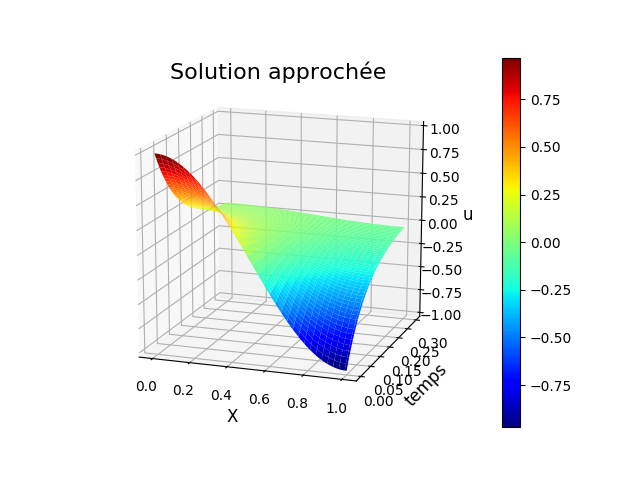
\includegraphics[scale=0.5]{./figure_1.png}\\


\subsection{Euler implicite}
Par le même raisonnement que pour Euler explicite, en prenant pour la dérivée en espace:\\

$$ \frac{u_{k} ^{n} - u_{k} ^{n-1}}{ \Delta t} - \frac{1}{( \Delta x)^2} (a_{k+\frac{1}{2}} u_{k+1}^n -(a_{k+\frac{1}{2}} +a_{k-\frac{1}{2}}) u_k ^n + a_{k-\frac{1}{2}}u_{k-1} ^n ) = f_k ^n $$


Enfin, l'écriture matricielle obtenue est:\\

$$ (Id - A)U^n = U^{n-1} + \Delta t F^n $$



\smallbreak

\section{Méthodes de travail}


Nous allons présenter dans cette partie comment nous avons travaillé en groupe afin de résoudre le projet.\\ 
\hspace*{1cm} Le problème rencontré est la différence de niveau en informatique au sein du groupe. Afin de surmonter ce problème, il a été décidé que nous résoudrons le projet par compétences. La partie programmation a été résolu par ceux qui avaient des compétences en informatiques. La partie théorique, comme la résolution de l'équation de la chaleur, et l'écriture du rapport a été élaboré par ceux qui ne savaient pas programmer. Il nous a paru clair que cette méthode était la plus efficace au niveau gain de temps. Le problème pouvant être la répartition de la charge de travail qui était affecté par les lacunes en informatique de certains membres du groupe.\\
















\section{Modèle}
\textbf{Le système linéaire du minimal model}, en dimension 1 :\\

\begin{equation}
\frac{\partial u}{\partial t}=\bigtriangledown( D \bigtriangledown U )-(J_{fi}+J_{so}+	J{si})
\end{equation}

\begin{equation}
\frac{\partial v}{\partial t}=\frac{(1-H(u-\theta_v)(v_\infty -v))}{\tau_v^-}-\frac{H(u-\theta_v)v}{\theta_v^+}
\end{equation}


\begin{equation}
\frac{\partial w}{\partial t}=\frac{(1-H(u-\theta_w)(w_\infty -w))}{\tau_w^-}-\frac{H(u-\theta_w)w}{\theta_w^+}
\end{equation}


\begin{equation}
\frac{\partial w}{\partial t}=\frac{\frac{1+tanh(k_s(u-u_s)}{2-s}}{\tau_s}
\end{equation}


Avec:


$J_si=\frac{-vH(u-\theta_v)(u-\theta_v)(u_u-u)}{\tau_{fi}}$

$J_so=\frac{\frac{u-u_0}{1-H(U-\theta_w)}}{\tau_{so}}$

$J_si=\frac{-H(u-\theta_w)ws}{\tau_{si}}$



Nous avons des représentations graphiques du minimal model après un codage en python :\\

Sur les quatres premières images nous avons choisit une simuation sur l'intervalle de temps : [5;6.5] ms\\


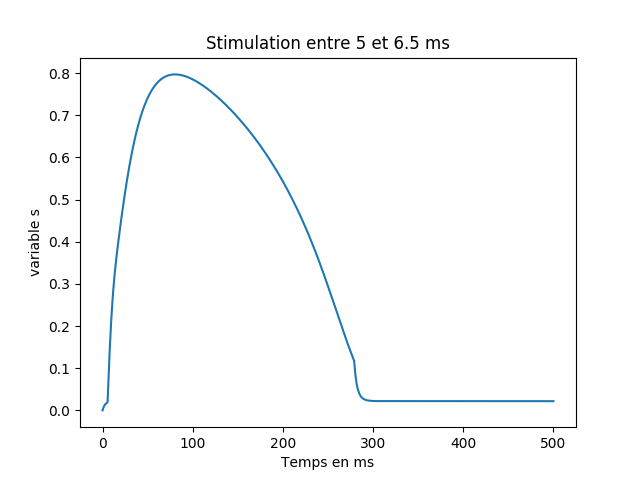
\includegraphics[scale=0.5]{./s(t).png}\\
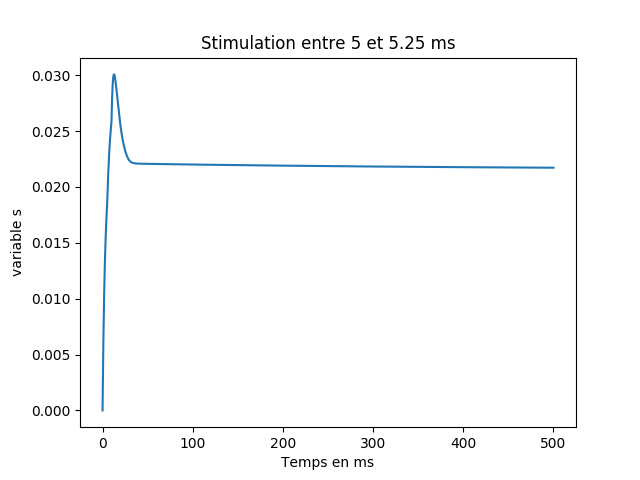
\includegraphics[scale=0.5]{./s(t)_2.png}\\
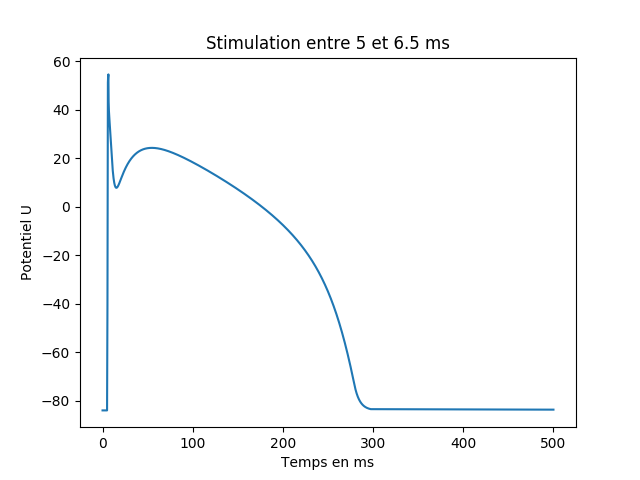
\includegraphics[scale=0.5]{./u(t).png}\\
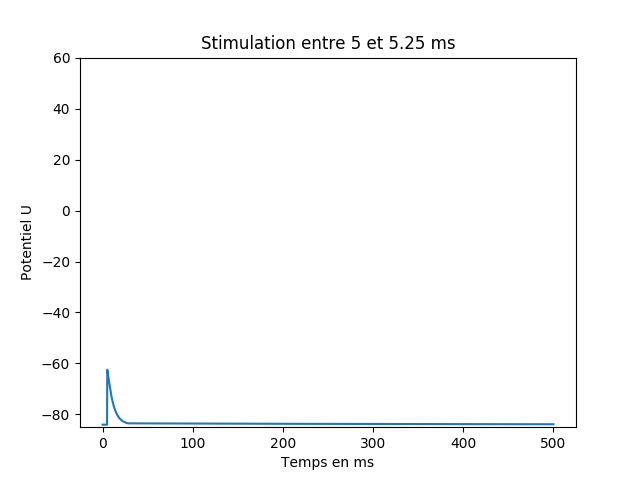
\includegraphics[scale=0.5]{./u(t)_2.png}\\
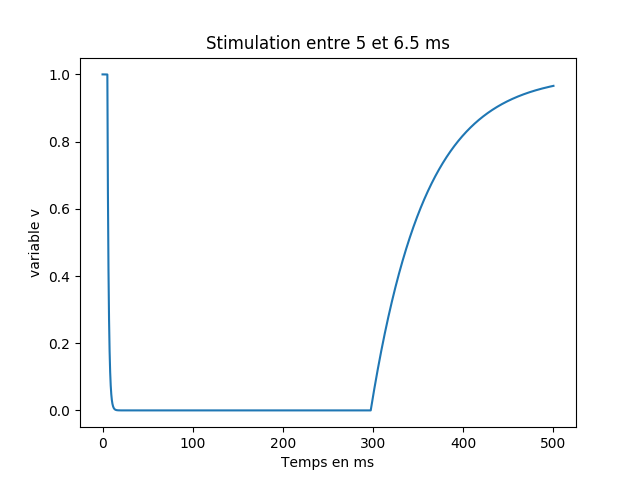
\includegraphics[scale=0.5]{./v(t).png}\\
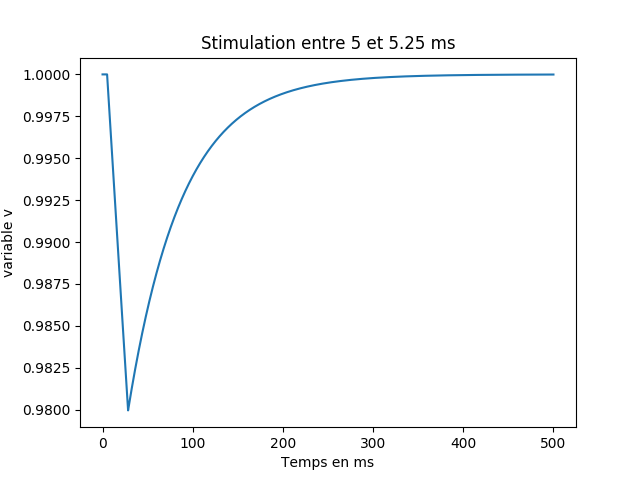
\includegraphics[scale=0.5]{./v(t)_2.png}\\
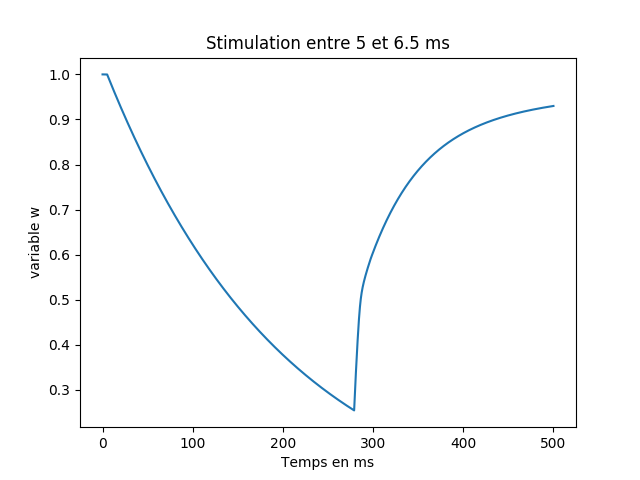
\includegraphics[scale=0.5]{./w(t).png}\\
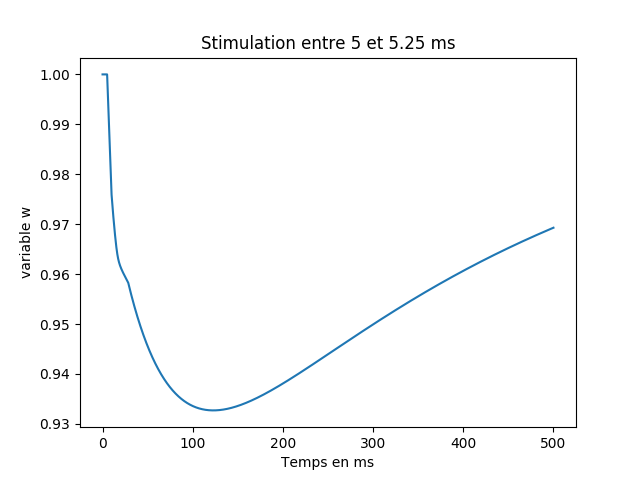
\includegraphics[scale=0.5]{./w(t)_2.png}\\





\underline{\textbf{Passage en dimension 2}}: 



Dans le passage en dimension en dimension 2 on se retrouve avec (l'équation ) , la variable a(x,y) devient une matrice $2*2$ .

Nous choisirons la matrice nommé A , diagonale composée de variables mesurables et positives :

 $\alpha(x,y)$ et $\beta(x,y)$

 

 le choix de ces  propriétés vient du fait que nous modélisons un phénomène de propagation ( du flux électrique qui travers les ventricule du cœur)


Notre matrice A sera ainsi de cette forme là:


\begin{equation}
A=\begin{pmatrix}\alpha(x,y)&0\\

0&\beta(x,y)\\\end{pmatrix}
 \end{equation}


Nous allons essayer de trouver les solutions analytiques de cette equation de dimension 2: 

\begin{equation}
\partial{t} u -\begin{pmatrix}\partial{x} & \partial{y}

\end{pmatrix} \begin{pmatrix}\alpha(x,y)&0\\

0&\beta(x,y)\\\end{pmatrix} \begin{pmatrix}\partial{x}u\\

\partial{y}u\\

\end{pmatrix} =f(x,y)
\end{equation}


On développe :

 

\begin{equation}
\partial{t} u -\begin{pmatrix}\partial{x} & \partial{y}

\end{pmatrix}\begin{pmatrix}\alpha \partial{x}U & \beta\partial{y} U

\end{pmatrix}=f(x,y)
\end{equation}

Et on se retrouve avec cette equation :

\begin{equation}
\partial{t} u-\partial{x}(\alpha \partial{x}U)-\partial{y}(\beta \partial{y}U)=f(x,y)
\end{equation}


Avec les conditions aux bords:

$\partial{x}U=\partial{y}U=0$

Nous allons maintenant appliquer le schéma d'Euler explicite 

\begin{equation}
\partial{t} (U{i,j} )^n=\frac{u_{i,j}^{n+1}-u_{i,j}^n}{\delta t}
\end{equation}

On applique les différences finies :

\begin{equation}
(\partial{x}(\alpha \partial{x}U))_{i,j}^n=\frac{\alpha_{i+1/2}^j\partial{x}U_{i+1/2}^n-\alpha_{i-1/2}^j\partial{x}U_{i-1/2}^n}{\delta x}=\alpha_{i+1/2}^j(\frac{U_{i+1,j}^n-U_{i,j}^n}{\delta^2})-\alpha_{i-1/2}^j(\frac{U_{i,j}^n-U_{i-1,j}^n}{\delta^2})
\end{equation}



\begin{equation}
\partial{x}(\alpha \partial{x}U)_{i,j}^n=\frac{\alpha_{i-1/2}^j}{\delta x^2}U_{i,j-1}^n+\frac{\alpha_{i+1/2}^j-\alpha_{i-1/2}^j}{\delta x^2}U_{i,j}^n +\frac{\alpha_{i+1/2}^j}{\delta x^2}U_{i+1,j}^n
\end{equation}



 Idem pour les dérivées partielles par apport à y : 

\begin{equation}
\partial{y}(\beta \partial{y}U)_{i,j}^n=\frac{\beta_i^{j-1/2}}{\delta y^2}U_{i,j-1}^n+\frac{\beta_{i}^{j+1/2}-\beta_{i}^{j-1/2}}{\delta y^2}U_{i,j}^n +\frac{\beta_{i}^{j+1/2}}{\delta y^2}U_{i,j+1}^n
\end{equation}



$i=1,....,N-1$


$j=1,....,N-1$


Du coup , 

\begin{equation}
\partial{t} (U{i,j} )^n -\partial{y}(\beta \partial{y}U)_{i,j}^n-\partial{x}(\alpha \partial{x}U)_{i,j}^n=f_i^j
\end{equation}

Donc on a comme schéma:

\begin{equation}
\frac{u_{i,j}^{n+1}-u_{i,j}^n}{\delta t}-\frac{\alpha_{i-1/2}^j  u_{i-1,j}^n +\beta_{i}^{j-1/2} u_{i,j-1}^{n}+ (\alpha_{i+1/2}^j - \alpha_{i-1/2}^j+ \beta_{i}^{j+1/2} -\beta_{i}^{j-1/2} ) u_{i,j}^n + \alpha_{i+1/2}^j u_{i+1,j}^{n} + \beta_{i}^{j+1/2} u_{i,j+1}^n}{h^2}=f_{i,j}
\end{equation}


Avec les conditions aux bords : 

\begin{equation}
\partial{x}(\alpha\partial{x}u)_{0,j}^n=0
\end{equation}


\begin{equation}
u_{0,j}^{n+1}=2\frac{\delta t}{\delta x^2}\alpha_{1/2}^j(u_{1,j}^n-u_{0,j}^n)f_0^j +u_{0,j}^n
\end{equation}


\begin{equation}
u_{N,j}^{n+1}=u_{N,j}^{n}+2\frac{\delta t}{\delta x} \alpha_{N-1/2}^j U_{N-1,j}^n-2\frac{\delta t}{\delta x} \alpha_{N-1/2}^j U_{N,j}^n +f_N^j
\end{equation}


\begin{equation}
u_{i,N}^{n+1}=u_{i,N}^{n}+2\frac{\delta t}{\delta x} \beta_{i}^{N-1/2} U_{i,N-1}^n-2\frac{\delta t}{\delta x} \beta_{i}^{N-1/2} U_{i,N}^n +f_i^N
\end{equation}


\begin{equation}
u_{i,0}^{n+1}=\frac{\delta t}{\delta x} \beta_{i}^{1/2}(U_{j,1}^n-U_{i,0}^n)j_j^0+U_{i,0}^n
\end{equation}


Pour coder, on pose A comme étant la matrice identité, et on fait une discrétisation uniforme  en espace $\delta x= \delta y = h$

\end{document}